\subsection{Az adattípus}
\noindent

Mielőtt belemélyedünk az paradigma központi elemeibe, nézzük meg, hogy hogyan specifikálunk egy típust. Erre azért lesz szükség, mert a típus specifikációja jól körülhatárolja majd azt, hogy milyen feladataink lesznek az objektumelvű kód tervezésekor.

\begin{figure}[H]
\centering
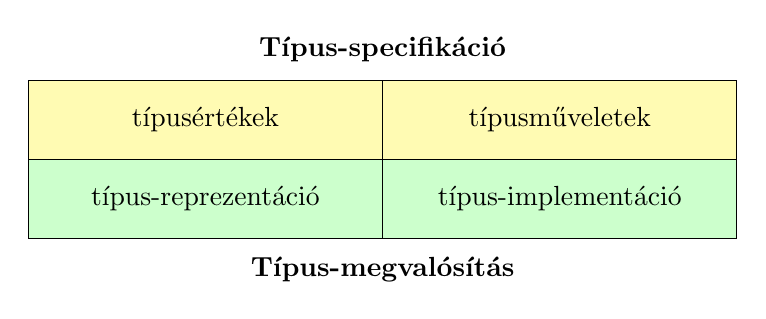
\begin{tikzpicture}
\def\cellwidth{4.5cm}
\def\cellheight{1cm}

\node at (\cellwidth, \cellheight + 0.4cm) {\textbf{Típus-specifikáció}};

\draw[fill=yellow!30] (0, 0) rectangle (\cellwidth, \cellheight);
\draw[fill=yellow!30] (\cellwidth, 0) rectangle (2*\cellwidth, \cellheight);
\draw[fill=green!20] (0, -\cellheight) rectangle (\cellwidth, 0);
\draw[fill=green!20] (\cellwidth, -\cellheight) rectangle (2*\cellwidth, 0);

\node at (0.5*\cellwidth, 0.5*\cellheight) {típusértékek};
\node at (1.5*\cellwidth, 0.5*\cellheight) {típusműveletek};
\node at (0.5*\cellwidth, -0.5*\cellheight) {típus-reprezentáció};
\node at (1.5*\cellwidth, -0.5*\cellheight) {típus-implementáció};

\node at (\cellwidth, -\cellheight - 0.4cm) {\textbf{Típus-megvalósítás}};
\end{tikzpicture}
\caption{Az adattípus felépítése}
\label{fig:adattipus}
\end{figure}

Az adattípus két komponensből áll, egy típus-specifikációból és egy típus-megvaló\-sí\-tás\-ból. A típus-specifikáció megadja az adat által felvehető értékek halmazát (\code{típusértékek}) és a típusértékekkel végezhető műveleteket (\code{típusműveletek}). A típus-megvalósítás megmutatja, hogy hogyan ábrázoljuk (\code{típus-reprezentáció}) a típusértékeket és milyen programok helyettesítsék (\code{típus-implementáció}) a műveleteket.

\bigskip
Tekintsük egy konkrét típus specifikációját, legyen ez a típus egy alma.

\begin{figure}[H]
\centering
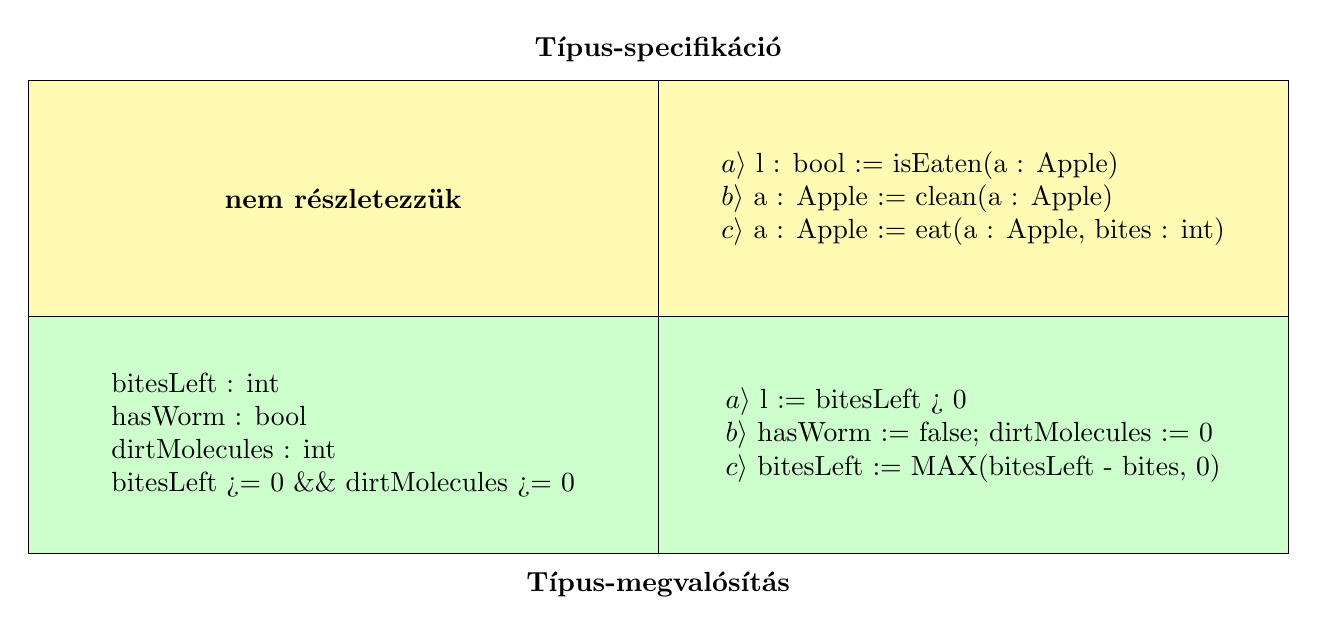
\begin{tikzpicture}
\def\cellwidth{8cm}
\def\cellheight{3cm}

\node at (\cellwidth, \cellheight + 0.4cm) {\textbf{Típus-specifikáció}};

\draw[fill=yellow!30] (0, 0) rectangle (\cellwidth, \cellheight);
\draw[fill=yellow!30] (\cellwidth, 0) rectangle (2*\cellwidth, \cellheight);
\draw[fill=green!20] (0, -\cellheight) rectangle (\cellwidth, 0);
\draw[fill=green!20] (\cellwidth, -\cellheight) rectangle (2*\cellwidth, 0);

\node[align=center] at (0.5*\cellwidth, 0.5*\cellheight) {\textbf{nem részletezzük}};
\node[align=left] at (1.5*\cellwidth, 0.5*\cellheight) {$a\rangle$ l : bool := isEaten(a : Apple)\\$b\rangle$ a : Apple := clean(a : Apple)\\$c\rangle$ a : Apple := eat(a : Apple, bites : int)};
\node[align=left] at (0.5*\cellwidth, -0.5*\cellheight) {bitesLeft : int\\hasWorm : bool\\dirtMolecules : int\\bitesLeft >= 0 \&\& dirtMolecules >= 0};
\node[align=left] at (1.5*\cellwidth, -0.5*\cellheight) {$a\rangle$ l := bitesLeft > 0\\$b\rangle$ hasWorm := false; dirtMolecules := 0\\$c\rangle$ bitesLeft := MAX(bitesLeft - bites, 0)};

\node at (\cellwidth, -\cellheight - 0.4cm) {\textbf{Típus-megvalósítás}};
\end{tikzpicture}
\caption{Az \code{Apple} adattípus}
\label{fig:apple-adattipus}
\end{figure}

Természetesen nem csak ez az egy lehetséges adattípus létezik egy alma modellezéséhez. A modell megalkotását az befolyásolja, hogy milyen műveleteket szeretnénk elvégezni egy almán. Ha például dobálni szeretnénk, akkor a tömegét is nyilván kellene tartani, és definiálni egy metódust, amely valamilyen $\theta$ szöget és valamilyen $F$ kifejtett erőt vár paraméterként.
\newpage